\documentclass[ignorenonframetext,]{beamer}
\setbeamertemplate{caption}[numbered]
\setbeamertemplate{caption label separator}{:}
\setbeamercolor{caption name}{fg=normal text.fg}

\usepackage{booktabs}
\usepackage{pifont}
\usepackage{ifxetex,ifluatex}
\usepackage{fixltx2e} % provides \textsubscript
\usepackage{lmodern}
\usepackage{algorithm}


\ifxetex
  \usepackage{fontspec,xltxtra,xunicode}
  \defaultfontfeatures{Mapping=tex-text,Scale=MatchLowercase}
  \newcommand{\euro}{€}
\else
  \ifluatex
    \usepackage{fontspec}
    \defaultfontfeatures{Mapping=tex-text,Scale=MatchLowercase}
    \newcommand{\euro}{€}
  \else
    \usepackage[T1]{fontenc}
    \usepackage[utf8]{inputenc}
      \fi
\fi
% use upquote if available, for straight quotes in verbatim environments
\IfFileExists{upquote.sty}{\usepackage{upquote}}{}
% use microtype if available
\IfFileExists{microtype.sty}{\usepackage{microtype}}{}

\providecommand{\tightlist}{%
  \setlength{\itemsep}{0pt}\setlength{\parskip}{0pt}}

% Comment these out if you don't want a slide with just the
% part/section/subsection/subsubsection title:
\AtBeginPart{
  \let\insertpartnumber\relax
  \let\partname\relax
  \frame{\partpage}
}
\AtBeginSection{
  \let\insertsectionnumber\relax
  \let\sectionname\relax
  \frame{\sectionpage}
}
\AtBeginSubsection{
  \let\insertsubsectionnumber\relax
  \let\subsectionname\relax
  \frame{\subsectionpage}
}

\setlength{\parindent}{0pt}
\setlength{\parskip}{6pt plus 2pt minus 1pt}
\setlength{\emergencystretch}{3em}  % prevent overfull lines
\setcounter{secnumdepth}{0}
\usepackage[english]{babel}
\usepackage{dsfont}
\usepackage{verbatim}
\usepackage{amsmath}
\usepackage{amssymb}
\usepackage{amsthm}
\usepackage{amsfonts}
\usepackage{csquotes}
\usepackage{multirow}
\usepackage{longtable}
\usepackage{enumerate}
\usepackage{bm}
\usepackage{bbm}
\usepackage{natbib}
% \usepackage[absolute,overlay]{textpos}
\usepackage{psfrag}
\usepackage{algorithm}
\usepackage{algpseudocode}
\usepackage{algpseudocodex}
\usepackage{float}
\usepackage{eqnarray}
\usepackage{arydshln}
\usepackage{tabularx}
\usepackage{placeins}
\usepackage{tikz}
\usepackage{setspace}
\usetikzlibrary{shapes,arrows,automata,positioning,calc}
\usepackage{subfig}
% \usepackage{paralist}
\usepackage{graphicx}
\usepackage{array}
\usepackage{framed}
\usepackage{excludeonly}
\usepackage{fancyvrb}
\usecolortheme{dove}
% \usefonttheme{serif}
\usepackage{xfrac}
\usepackage{xcolor}
\usepackage{mdframed}
\usepackage{caption}
\captionsetup[figure]{labelformat=empty}
\usepackage{transparent}

% URL color:
\definecolor{myorange}{RGB}{225, 127, 0}
% Theme color of metropolis
\definecolor{metropolis_theme_color}{RGB}{35,55,59}
% Upper and lower rules of code chunks
\definecolor{darkblue}{RGB}{34,55,58}
% Font color of footer:
\definecolor{mygrey}{RGB}{240,240,240}


%% %%%%%%%%%%%%%%%%%%%%%%%%%%%%%%%%%%%%%%%%%%%%%%%%%%%%%%%%%%%%%%%
%% METROPOLIS THEME + CUSTOMIZATIONS
%% %%%%%%%%%%%%%%%%%%%%%%%%%%%%%%%%%%%%%%%%%%%%%%%%%%%%%%%%%%%%%%%


\usetheme{metropolis}

%% Adjust frame number to be displayd as i/n:
%% ---------------------------------------------------------------
\setbeamertemplate{frame numbering}{%
  \insertframenumber{}/\inserttotalframenumber
}
\makeatother

\setbeamercolor{background canvas}{bg=white}

%% Add footer:
%% ---------------------------------------------------------------
\usepackage{framed, color}

\setbeamertemplate{footline}[text line]{%
    \noindent\hspace*{\dimexpr-\oddsidemargin-1in\relax}%
     \colorbox{metropolis_theme_color}{
     \makebox[\dimexpr\paperwidth-2\fboxsep\relax]{
     \color{mygrey}
     \begin{minipage}{0.33\linewidth}
       \secname
     \end{minipage}\hfill
     \begin{minipage}{0.33\linewidth}
       \centering
       \insertshortauthor
     \end{minipage}\hfill
     \begin{minipage}{0.33\linewidth}
       \flushright
       \insertframenumber{}/\inserttotalframenumber
     \end{minipage}
     }}%
  \hspace*{-\paperwidth}
}

%% Add titlegraphic:
%% ---------------------------------------------------------------
\titlegraphic{
  \vspace{3.5cm}
  \hspace{5.33cm}
  \transparent{0.2}
  
\includegraphics[width=8cm]{./style/images/logos/LMU}
}



%% %%%%%%%%%%%%%%%%%%%%%%%%%%%%%%%%%%%%%%%%%%%%%%%%%%%%%%%%%%%%%%%
%% NICER CODE BACKGROUND
%% %%%%%%%%%%%%%%%%%%%%%%%%%%%%%%%%%%%%%%%%%%%%%%%%%%%%%%%%%%%%%%%

% Define Shaded if not defined already through knitr:
%\definecolor{shadecolor}{RGB}{228,228,228}
\makeatletter
\@ifundefined{Shaded}{%
\newenvironment{Shaded}{\begin{snugshade}}{\end{snugshade}}%
}{}
\makeatother

\renewenvironment{Shaded}{
  \vspace{5pt}
  \begin{mdframed}[backgroundcolor=black!8,
                   linecolor=darkblue,
                   rightline=false,
				   leftline=false]}{
  \end{mdframed}}


%% %%%%%%%%%%%%%%%%%%%%%%%%%%%%%%%%%%%%%%%%%%%%%%%%%%%%%%%%%%%%%%%
%% CHANGE URL COLOR
%% %%%%%%%%%%%%%%%%%%%%%%%%%%%%%%%%%%%%%%%%%%%%%%%%%%%%%%%%%%%%%%%

\renewcommand\UrlFont{\color{myorange}}
% \hypersetup{
%     colorlinks=true,
%     linkcolor=myorange
% }

%% %%%%%%%%%%%%%%%%%%%%%%%%%%%%%%%%%%%%%%%%%%%%%%%%%%%%%%%%%%%%%%%
%% INCLUDE LATEX MATH + OTHER CUSTOMIZATIONS
%% %%%%%%%%%%%%%%%%%%%%%%%%%%%%%%%%%%%%%%%%%%%%%%%%%%%%%%%%%%%%%%%


% Include latex-math
\DeclareOldFontCommand{\sf}{\normalfont\sffamily}{\mathsf}

% \input{./../latex-math/basic-math.tex}
% \input{./../latex-math/basic-ml.tex}
% \input{./../latex-math/ml-bagging.tex}
% \input{./../latex-math/ml-boosting.tex}
% \input{./../latex-math/ml-gp.tex}
% \input{./../latex-math/ml-mbo.tex}
% \input{./../latex-math/ml-nn.tex}
% \input{./../latex-math/ml-svm.tex}
% \input{./../latex-math/ml-trees.tex}

% Additional commands:
% \newcommand{\abs}[1]{\ensuremath{\left| #1 \right|}}
% \renewcommand{\pikN}{\hat{\pi}^\Np} % This collides with z



% basic latex stuff
% \newcommand{\pkg}[1]{{\fontseries{b}\selectfont #1}} %fontstyle for R packages
% \newcommand{\lz}{\vspace{0.5cm}} %vertical space

\newcommand{\oneliner}[1] % Oneliner for important statements
{\begin{block}{}\begin{center}\begin{Large}#1\end{Large}\end{center}\end{block}}

\let\code=\texttt
\let\proglang=\textsf

\setkeys{Gin}{width=0.9\textwidth}

%% %%%%%%%%%%%%%%%%%%%%%%%%%%%%%%%%%%%%%%%%%%%%%%%%%%%%%%%%%%%%%%%
%% EXERCISE COUNTER
%% %%%%%%%%%%%%%%%%%%%%%%%%%%%%%%%%%%%%%%%%%%%%%%%%%%%%%%%%%%%%%%%

% Command for an automatic exercise counter for the exercise sheets:
\newcounter{Exercise}
\newcommand{\exercise}{
  \stepcounter{Exercise}
  \ifnum \theExercise = 1
    \Large{\textbf{Exercise \theExercise}} \\
  \else
    \vspace{\baselineskip} \Large{\textbf{Exercise \theExercise}} \\
  \fi
}

% Command for an automatic exercise counter for the courses:
\newcounter{CourseExercise}
\newcommand{\oneExercise}{
  \stepcounter{CourseExercise}
    \begin{center}
      \huge{Exercise \Roman{CourseExercise}}
    \end{center}
}
\newcommand{\twoExercises}{
  \stepcounter{CourseExercise}
    \begin{center}
      \huge{Exercise \Roman{CourseExercise} \& \stepcounter{CourseExercise} \Roman{CourseExercise}}
    \end{center}
}
\newcommand{\threeExercises}{
  \stepcounter{CourseExercise}
    \begin{center}
      \huge{Exercise \Roman{CourseExercise}, \stepcounter{CourseExercise} \Roman{CourseExercise} \& \stepcounter{CourseExercise} \Roman{CourseExercise}}
    \end{center}
}

\newcommand{\resetExercises}{\setcounter{CourseExercise}{0}}

\usetikzlibrary{shapes,arrows,automata,positioning,calc,chains,trees, shadows}
\tikzset{
  %Define standard arrow tip
  >=stealth',
  %Define style for boxes
  punkt/.style={
    rectangle,
    rounded corners,
    draw=black, very thick,
    text width=6.5em,
    minimum height=2em,
    text centered},
  % Define arrow style
  pil/.style={
    ->,
    thick,
    shorten <=2pt,
    shorten >=2pt,}
}
\usepackage{subfig}


\renewcommand{\mathbf}{\bm}
\newcommand*{\tran}{{\mkern-1.5mu\mathsf{T}}}

\newcommand{\D}{\mathcal{D}}
\newcommand{\fh}{\hat{f}}
\newcommand{\fmh}{\fh^{[m]}}
\newcommand{\fmdh}{\fh^{[m-1]}}
\newcommand{\blk}{k}
\newcommand{\blK}{K}
\newcommand{\tb}{\bm{\theta}}
\newcommand{\tbh}{\hat{\bm{\theta}}}
\newcommand{\tbmh}{\hat{\bm{\theta}}^{[m]}}
\newcommand{\tbih}[1][i]{\tbh^{(#1)}}
\newcommand{\xv}{\bm{x}}
\newcommand{\pr}{r}
\newcommand{\prv}{\bm{r}}
\newcommand{\rmi}{\pr^{[m](i)}}
\newcommand{\pd}[2]{\frac{\partial #1}{\partial #2}}
\renewcommand{\xi}[1][i]{\xv^{(#1)}}
\newcommand{\yi}[1][i]{y^{(#1)}}
\newcommand{\Lxyi}{L(\yi, f(\xi))}
\newcommand{\design}{\bm{Z}}
\newcommand{\sse}{\operatorname{SSE}}
\newcommand{\argmin}{\operatorname{arg~min}}
\newcommand{\riske}{\mathcal{R}_{\text{emp}}}
\newcommand{\rmm}{\prv^{[m]}}


\title{Accelerated component-wise gradient boosting using efficient data
representation and momentum-based optimization}
\author{D. Schalk, B. Bischl, D. Rügamer}
\date{17th, Dec.~2022}

\begin{document}
\begin{frame}[plain]
\titlepage
\end{frame}


\hypertarget{background}{%
\section{Background}\label{background}}

\begin{frame}{About the project}
\protect\hypertarget{about-the-project}{}
\begin{itemize}
\tightlist
\item
  Component-wise boosting
  \citep[CWB;][]{buhlmann2003boosting,buhlmann2007boosting} is a
  boosting method based on multiple base learners.
\item
  Utilizing interpretable statistical models as base learners makes the
  fitted model interpretable.
\item
  Also, CWB is can fit models in high dimensional features spaces and
  provides an inherent (unbiased) feature selection.
\item
  But, depending on the size of the data, it is infeasible to fit the
  algorithm w.r.t runtime or memory allocation.
\end{itemize}

\begin{itemize}
\item[$\Rightarrow$] \textbf{Goal:} Fasten the fitting process and reduce the memory consumption without loosing predictive or estimation accuracy.
\end{itemize}
\end{frame}

\begin{frame}{CWB basics I}
\protect\hypertarget{cwb-basics-i}{}
\begin{itemize}
\tightlist
\item
  Feature vector \(\bm{x} = (x_1, \dots, x_p)\in\mathcal{X}\)
\item
  CWB fits a model \(\fh\) based on an additive structure
  \[\mathbb{E}[Y|\bm{x}] = \fh(\bm{x}) = f_0 + \sum_{k=1}^K b_k(\bm{x}).\]
  Hence, CWB can be used as fitting engine for GAMs.
\item
  \(K\) additive terms represented by base learner
  \(b_k : \mathcal{X} \to \mathbb{R}\). Often one base learner per
  feature is used to model univariate effects.
\end{itemize}
\end{frame}

\begin{frame}{CWB basics II}
\protect\hypertarget{cwb-basics-ii}{}
\begin{itemize}
\tightlist
\item
  Example throughout the talk:

  \begin{itemize}
  \tightlist
  \item
    Three features \(x_{\text{age}}\), \(x_{\text{country}}\), and
    \(x_{\text{income}}\)
  \item
    Response \(Y\) is a numeric score for ``happiness''
  \item
    Aim: Model \(Y\) with \(b_{\text{age}}\) a P-spline,
    \(b_{\text{income}}\) a P-spline and \(b_{\text{country}}\) a
    one-hot encoding
  \end{itemize}
\end{itemize}

\begin{center}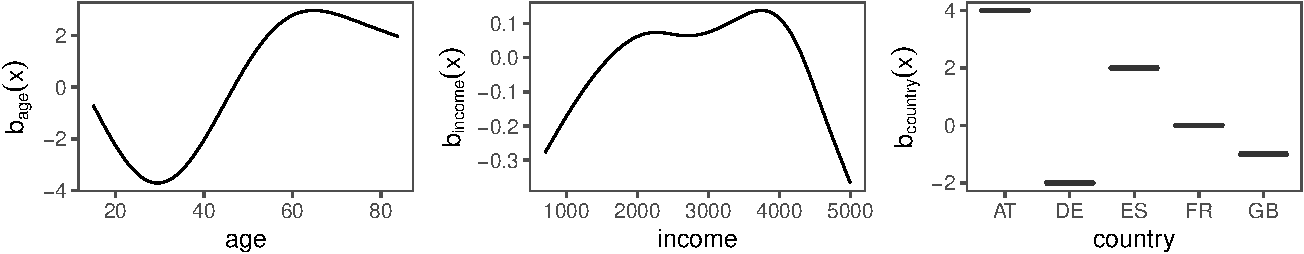
\includegraphics{figures/unnamed-chunk-1-1} \end{center}
\end{frame}

\begin{frame}{CWB algorithm I}
\protect\hypertarget{cwb-algorithm-i}{}
\begin{itemize}
\tightlist
\item
  Given is a data set \(\D\) with \(n\) observations and \(p\) features,
  a loss function \(L(y, \hat{y})\), and a set of base learners
  \(b_1, \dots, b_\blK\).
\item
  The gaol of fitting CWB is to minimize the empirical risk
  \(\riske(\fh | \D) = n^{-1}\sum_{(x,y)\in\D} L(y, \fh(x))\).
\item
  The algorithm is initialized with a loss-optimal constant \(c\) that
  minimizes the empirical risk:
  \[f_0 = \fh^{[0]}(\xv) = \argmin_{c\in\mathcal{Y}}\riske(c|\D)\]
\item
  Model updates are calculated by functional gradient descent:
  \[\fh^{[m+1]} = \fmh + \nu \hat{b}^{[m]}\]
\end{itemize}
\end{frame}

\begin{frame}{CWB algorithm II}
\protect\hypertarget{cwb-algorithm-ii}{}
\begin{itemize}
\tightlist
\item
  The negative functional gradient is expressed by pseudo residuals:
  \[\rmi = -\nabla_f L(y^{(i)}, f(\xi))|_{f = \fmdh},\ i \in \{1, \dots, n\}\]
\item
  In CWB, each base learner \(b_1, \dots, b_K\) is fitted to \(\rmm\)
  and the one with the lowest sum of squared errors (SSE) is chosen as
  new component \(\hat{b}^{[m]}\).
\item
  The last two step are repeated \(M\) times.
\end{itemize}
\end{frame}

\begin{frame}{CWB algorithm III}
\protect\hypertarget{cwb-algorithm-iii}{}
\begin{algorithm}[H]

\footnotesize

\caption{Vanilla CWB algorithm}\label{algo:cwb}
\vspace{0.15cm}
\hspace*{\algorithmicindent} \textbf{Input} Train data $\D$, learning rate $\nu$, number of boosting iterations $M$, loss\\
\hspace*{\algorithmicindent} \phantom{\textbf{Input} } function $L$, base learners $b_1, \dots, b_\blK$\\
\hspace*{\algorithmicindent} \textbf{Output} Model $\fh = \hat{f}^{[M]}$, estimated coefficient vectors $\tbih{1}, \ldots, \tbih{M}$\vspace{0.15cm}
\hrule

\begin{algorithmic}[1]
\Procedure{$\operatorname{CWB}$}{$\D,\nu,L,b_1, \dots, b_\blK$}
    \State Initialize: $f_0 = \fh^{[0]}(\xv) = \argmin_{c\in\mathcal{Y}}\riske(c|\D)$
    \While{$m \leq M$}
        \State $\rmi = -\left.\pd{\Lxyi}{f(\xi)}\right|_{f = \fmdh},\ \ \forall i \in \{1, \dots, n\}$%\label{algo:cwb:line:pr}
        \For{$\blk \in \{1, \dots, \blK\}$}
            \State $\tbmh_\blk = \left(\design_\blk^\tran \design_\blk + \bm{K}_\blk\right)^{-1} \design^\tran_\blk \rmm$%\label{algo:cwb:line:fitbl}
            \State $\sse_\blk = \sum_{i=1}^n(\rmi - b_\blk(\xi | \tbmh_\blk))^2$% \label{algo:cwb:line:sse}
        \EndFor
        \State $\blk^{[m]} = \argmin_{\blk\in\{1, \dots, \blK\}} \sse_\blk$% \label{algo:cwb:line:blselection}
        \State $\fmh(\xv) = \fmdh(\xv) + \nu b_{\blk^{[m]}} (\xv | \tbmh_{\blk^{[m]}})$
    \EndWhile
    \State \textbf{return} $\fh = \fh^{[M]}$
\EndProcedure
\end{algorithmic}
\end{algorithm}
\end{frame}

\begin{frame}{CWB advantages}
\protect\hypertarget{cwb-advantages}{}
\begin{itemize}
\tightlist
\item
  Can be fit in high dimensional feature spaces (\(n \ll p\)).
\item
  Variable selection (unbiased).
\item
  Estimation of partial feature effect that allows an interpretation of
  the final model.
\end{itemize}
\end{frame}

\begin{frame}{Goal}
\protect\hypertarget{goal}{}
For bigger data sets it is often infeasible to fit CWB.

\(\Rightarrow\) Increase CWB's efficiency:

\begin{itemize}
\tightlist
\item
  \textbf{Acceleration:} Fasten the fitting by using other optimizer.
\item
  \textbf{Memory:} Reduce the memory consumption.
\end{itemize}
\end{frame}

\hypertarget{acceleration}{%
\section{Acceleration}\label{acceleration}}

\begin{frame}{Nesterovs momentum}
\protect\hypertarget{nesterovs-momentum}{}
\textbf{Gradient descent:}

\vspace{0.2cm}
{\small
\begin{tabular}{ccc}
  Parameter space & & Functional space \\[0.3cm]
  $\tbh^{[m+1]} = \tbh^{[m]} + \nu \nabla_{\tb}\riske(\fh(. | \tbh^{[m]}) | \D)$ & $\Rightarrow$ & $\fh^{[m+1]} = \fmh + \nu \hat{b}^{[m]}$
\end{tabular}}
\vspace{0.2cm}

\textbf{Nesterov momentum:}

\vspace{0.2cm}
{\small
\begin{tabular}{ccc}
  Parameter space & & Functional space \\[0.3cm]
  $\bm{u}^{[m]} = \nabla_{\tb}\riske(\fh(. | \tbh^{[m]} - \gamma \hat{\bm{\vartheta}}^{[m-1]} | \D)$ &  & \\
  $\hat{\bm{\vartheta}}^{[m]} = \gamma \hat{\bm{\vartheta}}^{[m-1]} + \nu \bm{u}^{[m]}$ & $\Rightarrow$ & ??? \\
  $\tbh^{[m+1]} = \tbh^{[m]} + \hat{\bm{\vartheta}}^{[m]}$ & &
\end{tabular}}
\vspace{0.2cm}

\(\Rightarrow\) \textbf{Idea:} Use Nestervos momentum and adjust it for
functional updates and CWB.
\end{frame}

\begin{frame}{Nesterovs momentum in function space}
\protect\hypertarget{nesterovs-momentum-in-function-space}{}
\begin{itemize}
\tightlist
\item
  \citet{biau2019accelerated} proposed an adjustment of gradient
  boosting with Nesterovs momentum as optimizer.
\item
  \citet{lu2020accelerating} lined out that this approach may diverge
  and proposed an corrected algorithm Accelerated Gradient Boosting
  Machine (AGBM):
\end{itemize}

\vspace{-0.9cm}
\begin{align*}
g^{[m]} &= (1 - \theta_m) f^{[m]} + \theta_m h^{[m]}\\
f^{[m+1]} &= g^{[m]} + \eta b^{[m]} \\
h^{[m+1]} &= h^{[m]} + \eta / \theta_m b^{[m]}_{\text{cor}}
\end{align*}

with \(\theta_m = 2 / (m + 1)\) and \(h^{[m]}\) the momentum sequence.
\end{frame}

\begin{frame}{Base learners in AGBM}
\protect\hypertarget{base-learners-in-agbm}{}
\begin{itemize}
\tightlist
\item
  \(b^{[m]}\) is fit to pseudo residuals \(\rmm\) w.r.t.
  \(\hat{g}^{[m-1]}\) instead of \(\fmh\)
\item
  \(b^{[m]}_{\text{cor}}\) is fit to error-corrected pseudo residuals:
  \[c^{[m](i)} = \rmi + \frac{m}{m+1}(c^{[m-1](i)} - \hat{b}_{\text{cor}}^{[m-1]}(\xi)),\]
  with \(i = 1, \dots, n\), if \(m > 1\) and \(\bm{c}^{[m]} = \rmm\) if
  \(m = 0\).
\end{itemize}
\end{frame}

\begin{frame}{Adapting AGBM for CWB}
\protect\hypertarget{adapting-agbm-for-cwb}{}
In \citet{schalk2022accelerated}, we proposed an accelerated CWB (ACWB)
version by incorporating these adaptions to CWB, therefore:

\begin{itemize}
\tightlist
\item
  Both base learners, \(b^{[m]}\) and \(b^{[m]}_{\text{cor}}\), are the
  result of a selection process that chooses one of \(b_1, \dots, b_K\)
  w.r.t. to the minimal SSE on the respective pseudo residuals \(\rmm\)
  and \(\bm{c}^{[m]}\).
\item
  Update the estimated parameters accordingly to allow the estimation of
  partial feature effects.
\end{itemize}

Considering these issues allows to maintain all advantages of CWB in
ACWB. We refer to the publication for details about the algorithms.
\end{frame}

\begin{frame}{Hybrid CWB}
\protect\hypertarget{hybrid-cwb}{}
\begin{itemize}
\tightlist
\item
  We observed, that ACWB can overfit if not stopped early.
\item
  Therefore, we combined ACWB with CWB to accelerate the fitting in the
  beginning and fine-tune the model using CWB:
\end{itemize}

\begin{figure}
\centering
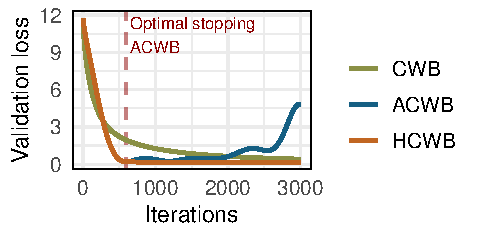
\includegraphics[width=0.7\textwidth]{figures/fig-optim-emp-risk.pdf}
\end{figure}
\end{frame}

\hypertarget{memory}{%
\section{Memory}\label{memory}}

\begin{frame}{Base learner design matrix}
\protect\hypertarget{base-learner-design-matrix}{}
\begin{itemize}
\tightlist
\item
  Each base learner \(b_1, \dots, b_K\) requires to build a design
  matrix \(\bm{Z}_k\in\mathbb{R}^{n\times d_k}\) based on the feature
  vector \(\bm{x}_k\).
\item
  For example:
\end{itemize}

\vspace{-0.4cm}
\begin{minipage}{0.75\textwidth}
{\tiny $
\bm{Z}_{\text{age}} = \begin{pmatrix}
    0 & 0 & 0 & 0 & 0 & 0 & 0  \\
    0.02 & 0.45 & 0.51 & 0.03 & 0 & 0 & 0 \\
    & & & \vdots & & & \\
    0.13 & 0.66 & 0.21 & 0 & 0 & 0 & 0 \\
    & 0 & 0 & 0 & 0.03 & 0.53 & 0.43 & 0.01
\end{pmatrix}
$}\hspace{0.2cm}{\Large $\Rightarrow$}
\end{minipage}
\begin{minipage}{0.2\textwidth}
\phantom{a}\vspace{0.4cm}\hspace*{0.5cm}

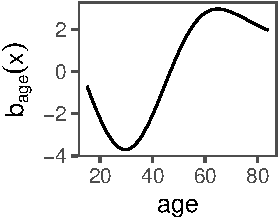
\includegraphics[width=3cm]{figures/unnamed-chunk-2-1} 
\end{minipage}

\(\Rightarrow\) If \(n\) is large, the memory gets filled very fast.
\end{frame}

\begin{frame}{Binning}
\protect\hypertarget{binning}{}
\begin{itemize}
\tightlist
\item
  To reduce the memory consumption, we applied binning to operate on a
  reduced representation of \(\bm{Z}_k\).
\item
  Binning is a technique that allows to represent the \(n\) values
  \(x_k^{(1)}, \dots, x_k^{(n)}\) of \(\xv_k\) by \(n^\ast < n\) design
  points \(\bm{z}_k = (z_k^{(1)}, \dots, z_k^{(n^\ast)})\).
\item
  The idea is to assign each \(x_k^{(i)}\) to the closest design point
  \(z_k^{(i)}\) and store the assignment in a map
  \(\text{ind}_k^{(i)}\):
  \(x_k^{(i)} \approx z_k^{(\text{ind}_k^{(i)})}\)
\end{itemize}

\begin{center}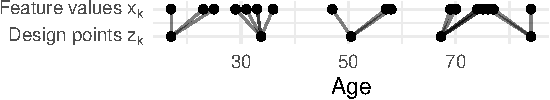
\includegraphics[width=9cm]{figures/unnamed-chunk-3-1} \end{center}
\end{frame}

\begin{frame}{Binning in GLMs}
\protect\hypertarget{binning-in-glms}{}
\begin{itemize}
\item
  \citet{lang2014multilevel} used binning to discretize feature vectors
  to increase the efficiency of multilevel structured additive
  regression.
\item
  \citet{wood2017gigadata} applied binning to fit GAMs to gigadata and
  argue that the best approximation is achieved by setting
  \(n^\ast = \sqrt{n}\).
\item
  \citet{li2020faster} presented optimized cross-product operations of
  design matrices based on binned features.
\item
  Besides the memory reduction, these operations further speed up the
  runtime.
\end{itemize}
\end{frame}

\begin{frame}{Binning in CWB}
\protect\hypertarget{binning-in-cwb}{}
\begin{itemize}
\tightlist
\item
  Represent numerical features \(\bm{x}_k\) by \(n^\ast\) design points
  \(\bm{z}_k\).
\item
  Build the design matrix \(\bm{Z}_k\) based on \(\bm{z}_k\) which
  requires to store \(n^\ast d_k\) values instead of \(nd_k\).
\item
  Use optimized cross-product operations to estimate the parameters
  \(\tbh_k^{[m]} = (\bm{Z}_k^\tran \bm{Z}_k + \bm{K}_k)^{-1}\bm{Z}_k^\tran \rmm\)
  of a base learner to also speed up the fitting.
\end{itemize}
\end{frame}

\hypertarget{application-to-data}{%
\section{Application to data}\label{application-to-data}}

\begin{frame}{Benchmark}
\protect\hypertarget{benchmark}{}
\begin{figure}
\centering
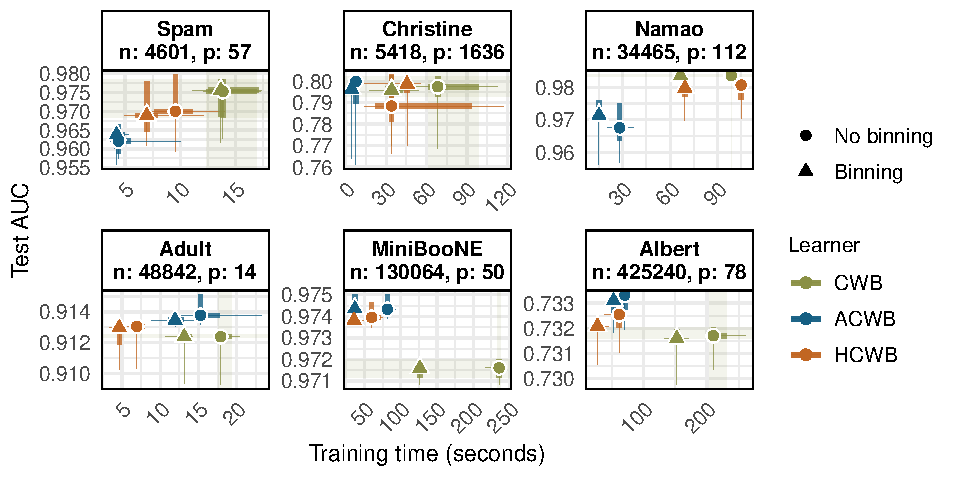
\includegraphics[width=\textwidth]{figures/fig-eq2-2.pdf}
\end{figure}
\end{frame}

\begin{frame}{Binning with big data}
\protect\hypertarget{binning-with-big-data}{}
\begin{itemize}
\tightlist
\item
  HIGGS: \(11 \times 10^6\) observations, \(29\) features, 2.4 GB
\item
  NYC Yellow Taxi Trip: \(24.3 \times 10^6\) observations, \(22\)
  features, 3.3 GB
\item
  FEMA's National Flood Insurance Policy Database: \(14.5 \times 10^6\)
  observations, \(50\) features, 3.4 GB
\end{itemize}

\begin{figure}
\centering
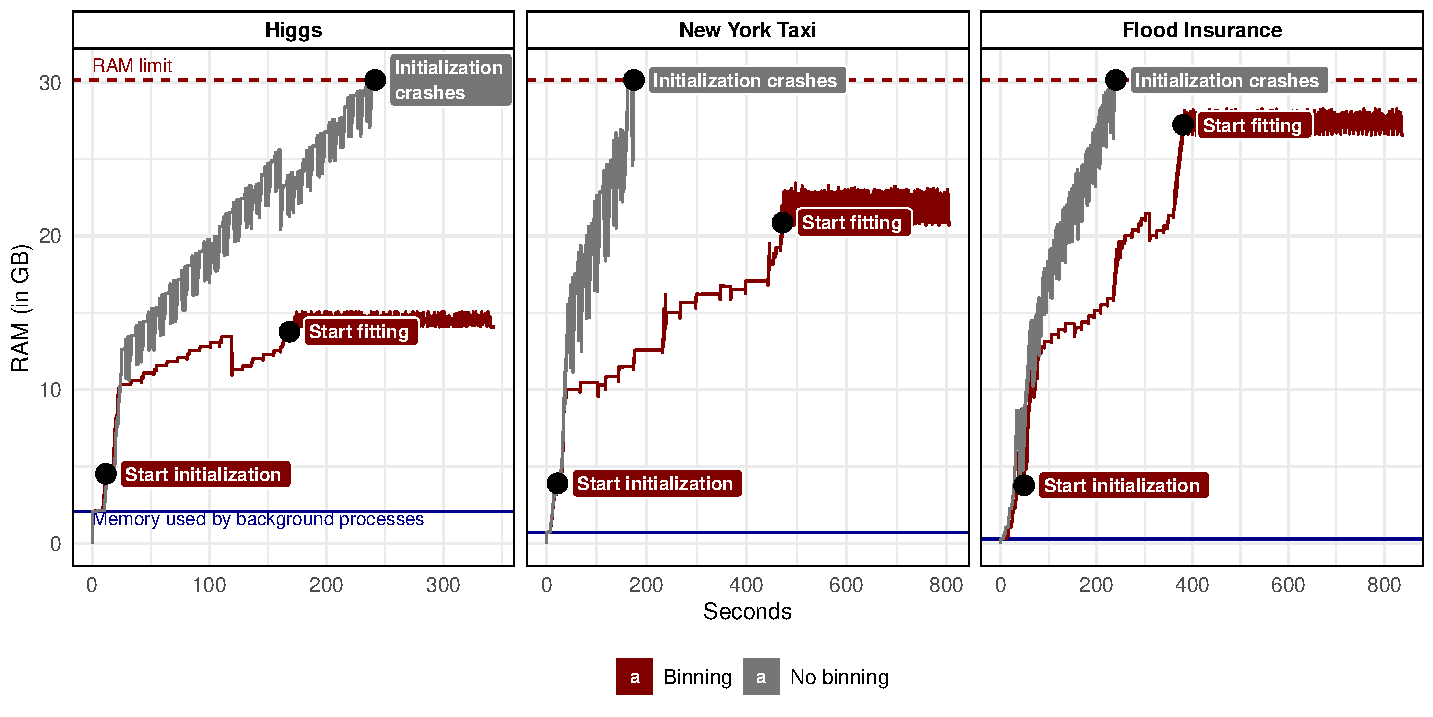
\includegraphics[width=0.8\textwidth]{figures/app-big-data.pdf}
\end{figure}
\end{frame}

\hypertarget{references}{%
\section{References}\label{references}}

\begin{frame}[allowframebreaks,plain]{}
\protect\hypertarget{section}{}
\footnotesize
\bibliographystyle{apalike}
\bibliography{references.bib}
\end{frame}

\end{document}
